%\subsection{Interactive in~transit visualization by staging data in a processing pipeline}

ADIOS provides a single I/O API for the simulation to output data, and a visualization tool to read input data. The codes are written as if writing the data to files and reading data from files, and they work in that mode too. ADIOS also provides methods to transfer data from the output to the reader(s) and thus allows for a seemless switch from file-based post-processing to online processing helped with memory-to-memory data transfers. Staging methods that transfer data from the memory of the producer into the memory of the consumer are best for coupling and for a straight analytical pipeline (e.g. DIMES \cite{ADIOS:DIMES-XXX} and FLEXPATH \cite{ADIOS:FLEXPATH-XXX}). The DataSpaces model~\cite{ADIOS:Docan:hpdc10}, however, provides a virtual shared multi-dimensional space using a set of separate nodes as a ``staging area,". Thus multiple, parallel applications can simultaneously read a multi-dimensional array, with an arbitrary decomposition. More importantly for interactive visualization, DataSpaces can hold as many output steps as the allocated memory can hold and can serve a reader with data the producer long has forgotten about. Moreover, DataSpaces provides fault isolation for the application. Failures downstream in a process pipeline does not propagate to the application. More details on using ADIOS and DataSpaces for in-transit visualization can be found in the book on High Performance Visualization~\cite{ADIOS:Bethel-Childs-Hansen:HPV:2012}.

A visualization pipeline is shown in Figure~\ref{part3-ch5-adios:fig:intransitviz}. Pixie3D \cite{ADIOS:Chacon:2002} is yet another fusion simulation code (of the magneto-hydrodynamic type). This code's output cannot directly be used for visualization because of its internal geometries optimized for execution performance, not for human friendly representation. A separate code, Pixplot, has always been used to process the output on a small number of processes, transform and write the data and multiple meshes in Cartesian coordinates, feasible for visualization. The three components in the visualization pipeline, Pixie3D simulation, Pixplot transformation and ParaView parallel visualization tool, represent a typical scenario for concurrent in~transit visualization. All these codes have already used ADIOS for writing and reading data for post run exploration, so it was easy to set them up for concurrent visualization. The only change in the application code was to change the processing loop in Pixplot, which has assumed in post-processing that the number of timesteps was known at the beginning of the processing. With in~transit processing, the code had to loop for an unknown amount of iterations as long as there was data coming from the simulation and to read a timestep from the the staging area, possibly waiting a bit if the next timestep is not yet available. The same was true for ParaView's ADIOS reader, which before had expected data in a file with all timesteps available.  

\begin{figure}[h!]
\centering
\myIfColor
{
% use color version
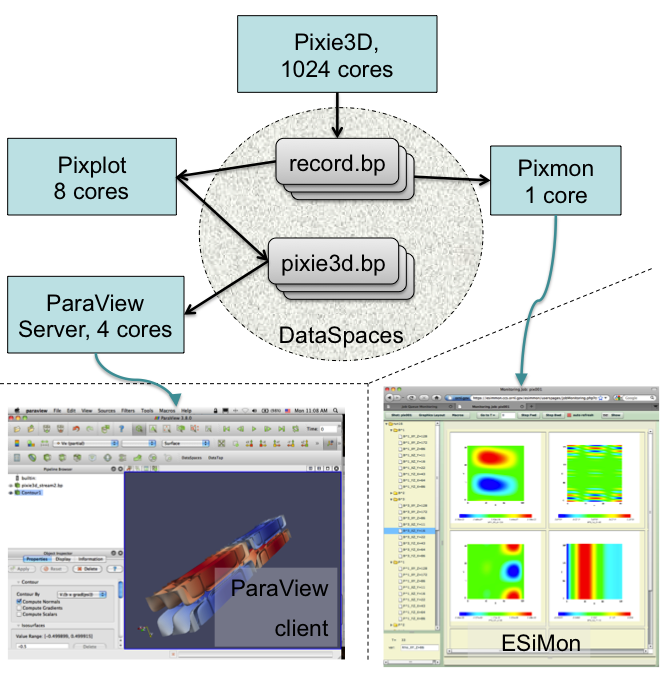
\includegraphics[width=0.6\textwidth]{Chapters/part3-ch5-adios/figs/intransitviz.png}
}
{
% use B&W version
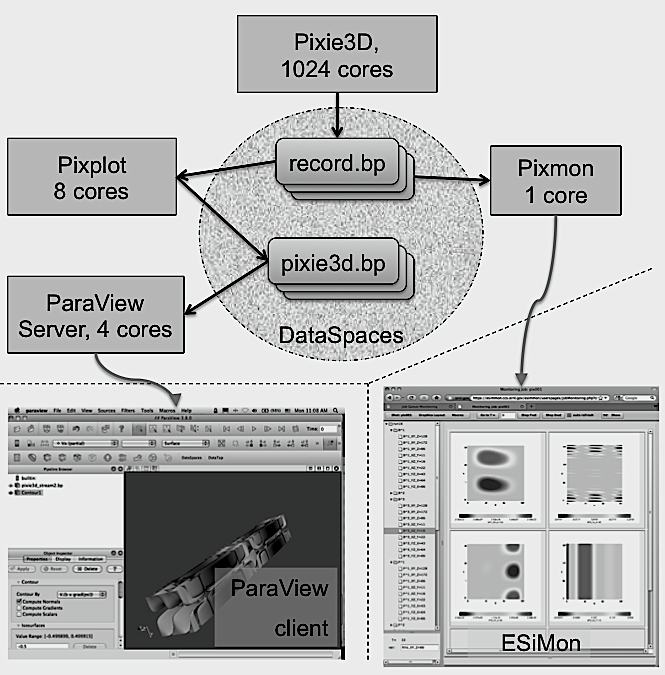
\includegraphics[width=0.6\textwidth]{Chapters/part3-ch5-adios/figs/intransitviz-bw.png}
}
\caption[]
{In~transit analysis and visualization pipeline using ADIOS and DataSpaces.
}
\label{part3-ch5-adios:fig:intransitviz}
\end{figure}

